\documentclass[10pt]{beamer}

\usetheme[progressbar=frametitle]{metropolis}
\usepackage{appendixnumberbeamer}
\usepackage{graphicx}	
\usepackage{booktabs}
\usepackage[scale=1]{ccicons}

\usepackage{pgfplots}
\usepgfplotslibrary{dateplot}

\usepackage{xspace}
\newcommand{\themename}{\textbf{\textsc{metropolis}}\xspace}

\title{Seminar}
\subtitle{Gitflow}
% \date{\today}
\date{}
\author{Dorian Janžetić, Antonio Babić, Antonio Puhanić}
\institute{Tehnički Fakultet Rijeka}
% \titlegraphic{\hfill\includegraphics[height=1.5cm]{logo.pdf}}

\begin{document}

\maketitle

\section{Uvod}
\begin{frame}{Gitflow}

Gitflow je posebna vrsta workflow-a.

Dizajniran je tako da striktno definira početne grane na kojemu se cijeli projekt bazira.

Pruža framework koji je efikasan za velike projekte, ili projekte koji imaju vremenski rok.

Stirktno definira ulogu svake grane.
\end{frame}
\begin{frame}{Gitflow}
Gitflow korsti sve normalne funkcije git-a uz svoje nadogradnje.

U gitflow projektima se definira pojedinačna grana za sve.

Npr: \textit{bugfix},\textit{hotfix}, \textit{feature} i sl.

Glavna grana na kojoj se radi je \textit{develop} i na nju se nadovezuju ostale grane poput vec navedenih.

Kada je projekt spreman, \textit{develop} grana se spaja u \textit{master} granu

\end{frame}
\begin{frame}{Gitflow}
Da bi se uopće moglo raditi na projektu uz Gitflow potrebno ga je prvo instalirati.

Jer je to zapravo nadogradnja na postojeći Git.

Instalacija je jednostavna, za OSX sisteme se može koristiti naredba \textit{brew install git-low}, a za Windows OS klasičnim preuzimanjem i instaliranjem.

Za inicijaizaciju Gitflow projekta umjesto \textit{git init}, koristi se \textit{git flow init}.

Ne mijenja ništa u projektu osim što stvara unaprijed definirane grane.
\end{frame}
\begin{frame}{Gitflow grane}
Umjesto uobičajene jedne glavne \textit{master} grane, Gitflow koristi dvije.
Druga je \textit{develop} grana.

{
\setlength{\fboxsep}{1pt}
\setlength{\fboxrule}{1pt}
\fbox{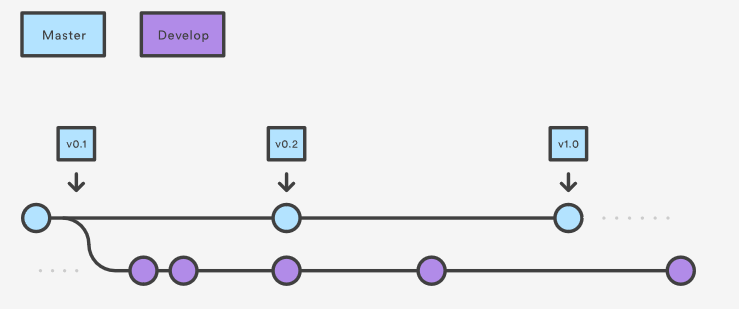
\includegraphics[width=11cm, height=4cm]{master_develop}}
}

\end{frame}
\begin{frame}{Gitflow grane}
\textit{Develop} grana je ona na kojoj se odvija većina projekta, iz koje se stvaraju i vraćaju nove grane.

Za objavljivanje tj. završavanje projekta sve se spaja u \textit{develop} granu.

Zbog ovog načina workflow-a poželjno je svaku objavu ili commit tagirati.

Ovako se bilježi cijela povijest razvoja projekta ili programa.

Na repozitoriju treba postojati develop grana koju svi developeri prate.

\end{frame}

\begin{frame}{Feature grana}

Kad god radimo na novoj značajci (\textit{featureu}) stvaramo novu \textit{Feature} granu koja se grana iz \textit{Develop} grane. Kada napravimo značajku spajmo ju sa \textit{Develop} granom.
Feature grane se \textbf{nikad] ne spajaju direktno u master granu.

{
\setlength{\fboxsep}{1pt}
\setlength{\fboxrule}{1pt}
\fbox{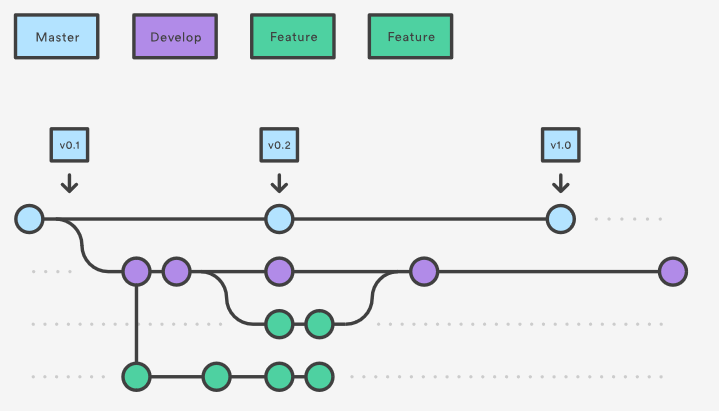
\includegraphics[width=10cm, height=4cm]{feature}}
}

\end{frame}

\begin{frame}{Korištenje feature grane}

ako nemamo git-flow ekstenzije:
Stvaranje grane:
git checkout develop
git merge feature_branch
Spajanje grane:
git checkout develop
git merge feature_branch

ako imamo git-flow ekstenzije:
Stvaranje grane:
git flow feature start feature_branch
Spajanje grane:
git flow feature finish feature_branch

\end{frame}

\begin{frame}{Release grana}

Kada smo blizu izdavanju nove verzije \textit{forkanjem} \textit{Develop} grane stvaramo \textit{Release} granu.
U ovu granu se smiju dodavati samo \textit{bug fixovi} i dokumentacija vezana za izdavanje nove verzije. Ne smiju se dodavati nikakve nove značajke.

{
\setlength{\fboxsep}{1pt}
\setlength{\fboxrule}{1pt}
\fbox{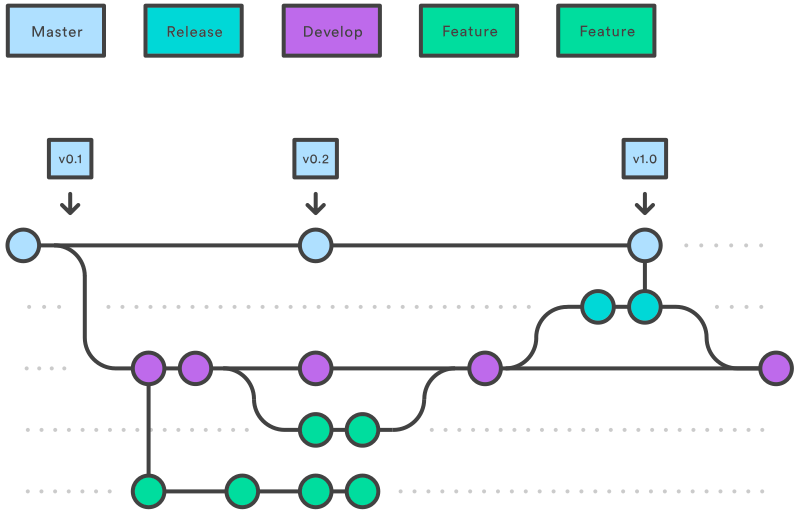
\includegraphics[width=9cm, height=4.5cm]{release}}
}

\end{frame}

\begin{frame}{Release grana}

Prednost ovakvog pristupa je u tome što dio tima može nastaviti raditi na značajkama za sljedeću verziju dok drugi dio tima dovršava detalje vezane uz verziju koja uskoro izlazi.
Kada dovršimo \textit{Release} granu spajamo ju i s \textit{Master} i s \textit{Develop} granom. S \textit{Develop} granom ju spajamo jer je moguće da smo dodali bitna ažuriranja na \textit{Release} granu koja želimo imati uključena u daljni razvoj projekata.

\end{frame}


\begin{frame}{Korištenje feature grane}

ako nemamo git-flow ekstenzije:
Stvaranje grane:
git checkout develop
git checkout -b release/0.1.0
Spajanje grane:
git checkout develop
git merge release/0.1.0

ako imamo git-flow ekstenzije:
Stvaranje grane:
$ git flow release start 0.1.0
Switched to a new branch 'release/0.1.0'
Spajanje grane:
git checkout master
git checkout merge release/0.1.0
git flow release finish '0.1.0'

\end{frame}

\begin{frame}{Hotfix grana}
Još jedna vrsta grane u Gitflow-u je \textit{hotfix} grana, te služi za održavanje ili hitne izmjene.

\textit{Hotfix} grana je slična \textit{release} ili \textit{feature} grani, samo što se bazira na \textit{master} grani umjesto \textit{develop} grani.

Nakon što je popravak ili izmjena gotova \textit{hotfix} grana se spaja (merge) sa \textit{master} i \textit{develop} granama, te \textit{master} grana dobiva novi broj verzije.
{
\setlength{\fboxsep}{1pt}
\setlength{\fboxrule}{1pt}
\fbox{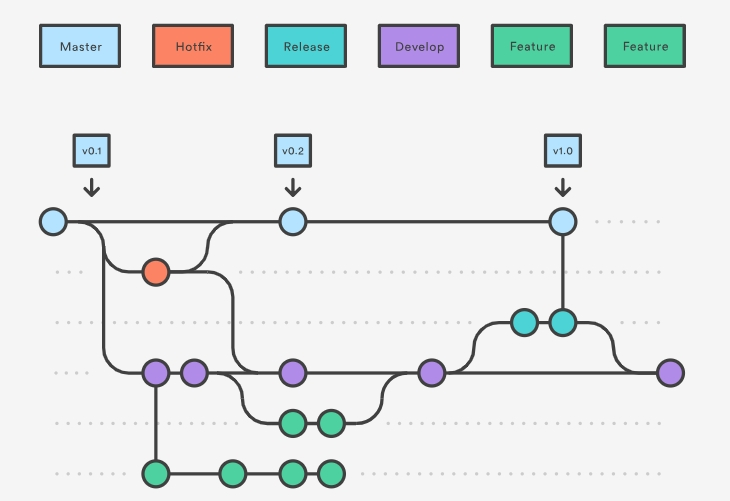
\includegraphics[width=9cm, height=4.5cm]{hotfix}}
}
\end{frame}
\begin{frame}{Korištenje hotfix grane}
Ako želimo napraviti \textit{hotfix} granu, možemo na 2 načina ovisno imamo li git-flow ekstenziju:

- bez git-flow ext.: \textbf{git checkout master}

\textbf{git checkout -b hotfix\_branch}
                         
- sa git-flow ext.:  \textbf{git flow hotfix start hotfix\_branch}

Nakon što smo gotovi sa \textit{hotfix} granom samo ju spajamo sa drugim granama te ju nakon toga obrišemo.
\end{frame}
\begin{frame}{Ukratko gitflow}
Gitflow je izvrstan za korištenje kod razvijanja softwarea koji se bazira na izdanjima, tj. verzijama i ima zasebnu granu na kojoj se mogu vršiti mali popravci i izmjene,

Radni tijek u gitflow-u ukratko je:
\begin{enumerate}
    \item \textit{develop} grana se stvara od \textit{master} grane
    \item \textit{release} grana se stvara od \textit{develop} grane
    \item \textit{feature} grane se stvaraju od \textit{develop} grane
    \item Kada je novi \textit{feature} gotov spaja se u \textit{develop} granu
    \item Kada je \textit{release} gotov spaja se u \textit{develop} i \textit{master} grane
    \item Ako se nađe greška u \textit{master} grani onda se stvara nova \textit{hotfix} grana
    \item Kada je greška otklonjena u \textit{hotfix} grani, ponovno se spaja u \textit{master} i \textit{develop} grane
\end{enumerate}
\end{frame}
\end{document}
